\documentclass[tikz,border=5mm]{standalone}
\usepackage{amsmath,amsfonts,amssymb}
\usetikzlibrary{calc}
\begin{document}
	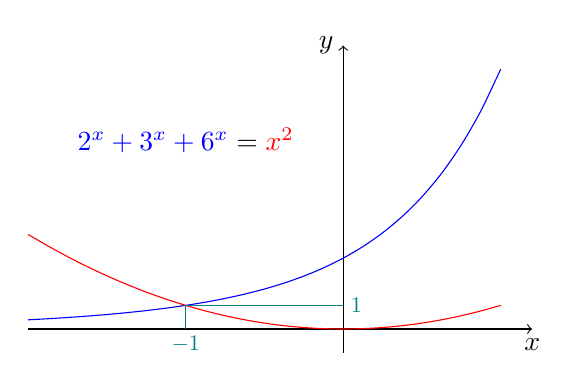
\begin{tikzpicture}[y=3mm,x=2cm]
		\draw[->] (-2,0)--(1.2,0) node[below]{$x$};
		\draw[->] (0,-1)--(0,12) node[left]{$y$};
		\draw[blue,smooth] plot[domain=-2:1] (\x,{pow(2,\x)+pow(3,\x)+pow(6,\x)});
		\draw[red,smooth] plot[domain=-2:1] (\x,{pow(\x,2)});
		\draw[very thin,teal]
		(0,1) node[right,scale=.8]{$1$}--(-1,1)
		(-1,0) node[below,scale=.8]{$-1$}--(-1,1)
		;
		\path (-1,8) node{{\color{blue}$2^x+3^x+6^x$}\;=\;{\color{red}$x^2$}};
	\end{tikzpicture}
\end{document}